\documentclass[11pt]{article}

\newcommand{\cnum}{CM146}
\newcommand{\ced}{Fall 2018}
\newcommand{\ctitle}[3]{\title{\vspace{-0.5in}\cnum, \ced\\Problem Set #1: #2}}
\usepackage{enumitem}
\newcommand{\solution}[1]{{{\color{black}{\bf Solution:} {#1}}}}
\usepackage[usenames,dvipsnames,svgnames,table,hyperref]{xcolor}
\usepackage{amsmath}
\usepackage{graphicx}

\renewcommand*{\theenumi}{\alph{enumi}}
\renewcommand*\labelenumi{(\theenumi)}
\renewcommand*{\theenumii}{\roman{enumii}}
\renewcommand*\labelenumii{\theenumii.}

\begin{document}
\ctitle{01}{Jonathan Chu}
\date{}
\maketitle
\vspace{-0.75in}

\section{(on CCLE)}
\section{Entropy and Information}
\begin{enumerate}
\item

\solution{
$$Gain(S, X_j) = Entropy(S) - \sum_{v \in V} \frac{|S_v|}{|S|}Entropy(S_v)$$
$$Gain(S, X_j) = B\left(\frac{p}{p+n}\right) - \sum_{v \in V} \frac{|S_v|}{|S|}B\left(\frac{p}{p+n}\right)$$
$$Gain(S, X_j) = B\left(\frac{p}{p+n}\right)\left(1 - \sum_{v \in V}\frac{|S_v|}{|S|}\right) = 0$$
}

\end{enumerate}

\section{k-Nearest Neighbors and Cross-validation}
\begin{enumerate}
\item %3a
\solution{Because a point is considered its own neighbor, the value of k that minimizes the training set error is 1. The resulting training error is 0, since our prediction will always equal the training example's value.}
\vspace{0.5cm}

\item %3b
\solution{
Since our task is binary \{-1, 1\}, a very large value of k would cause the average output of neighbors to be very close to 0, meaning our prediction will always be low confidence.
\newline
\newline
A very small value of k could result in overfitting, since we only consider very similar examples in the training set when making a prediction. Outliers in the training data would have more impact on our predictions.
}
\vspace{0.5cm}

\item %3c
\solution{
By inspection, there is no value of k for which we can correctly predict the 2 upper +'s and the 2 lower -'s in a leave-one-out setting. Thus, the minimum error we can hope to achieve is 4/14. Intuitively, we seek k values that encompass all or at least most of the other points in the same group of 7. 
\newline
\newline
Values of k that achieve this are 5 and 7. 6 is not guaranteed to achieve minimum error because, for example, (1, 5) is equidistant to both (5, 1) which is not the desired prediction, and (5, 9) which is.
}
\end{enumerate}

\section{Applying decision trees and k-nearest neighbors}
\begin{enumerate}
\item %4a
\solution{

Pclass:
The better the class, the greater the chance of survival. The 3rd class had a much lower frequency of survival than the other classes. Roughly 2/3 of first class members survived, and the 2nd class was fairly even between survivors and deaths.

Sex:
There is a large disparity in survival rate between men and women, women being more fortunate.

Age:
Children under ten had the highest survival rate. Otherwise, there isn’t an obvious trend.

Siblings/Spouses:
There weren’t many individuals with more than one sibling/spouse. Individuals with 1 sibling/spouse had the highest frequency of survival, and those with 0 had a rather low frequency of survival.

Parents/Children:
There were very few individuals with more than 2 parents/children. Those with 1-2 had a high frequency of survival, and those with 0 had lower rates.

Fare:
The majority of passengers paid a fare below 50, and these individuals had a rather low frequency of survival. All passengers who paid more had much greater survival rates.

Port of Embarkation:
Passengers who embarked from Cherbourg had a much higher frequency of survival than the other 2 ports.
}
\vspace{0.5cm}

\item %4b
\solution{
We set the probabilities to [occurrences of 0]/[length of y] and [occurrences of 1]/[length of y] for 0 and 1, respectively, and generate n random values from \{0, 1\} using those probabilities:

Classifying using Random...

	-- training error: 0.485
}
\vspace{0.5cm}

\item %4c
\solution{

Classifying using Decision Tree...

	-- training error: 0.014
}
\vspace{0.5cm}

\item %4d
\solution{

Classifying using k-Nearest Neighbors...

	-- training error for k=3: 0.167
	
	-- training error for k=5: 0.201
	
	-- training error for k=7: 0.240
}
\vspace{0.5cm}

\item %4e
\solution{
Investigating various classifiers...

	-- MajorityVote: training error = 0.400, test error = 0.403
	
	-- Random:       training error = 0.484, test error = 0.481
	
	-- DecisionTree: training error = 0.011, test error = 0.243
	
	-- KNeighbors:   training error = 0.210, test error = 0.311
}

\newpage
\item %4f
\solution{
Finding the best k for KNeighbors classifier...
	-- the value of k that minimizes cross validation error is 7
}

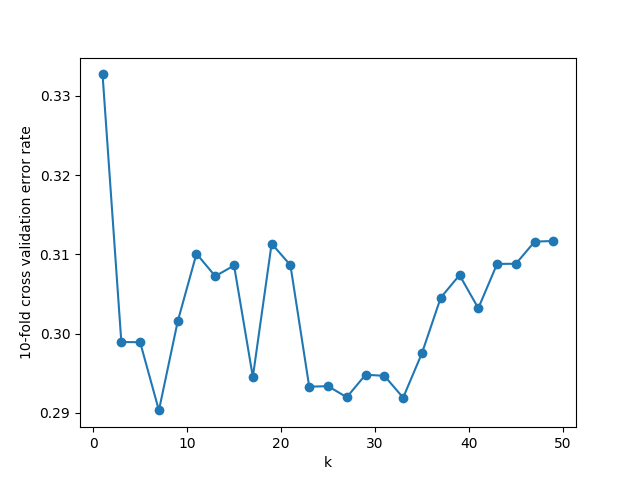
\includegraphics[width=\linewidth]{KNN-CV.png}

\newpage
\item %4g
\solution{
Investigating depths...

	-- the depth that minimizes cross validation error is 3
	
For larger depth values, there is clearly overfitting. The training error approaches zero, while the test error gradually increases.
}

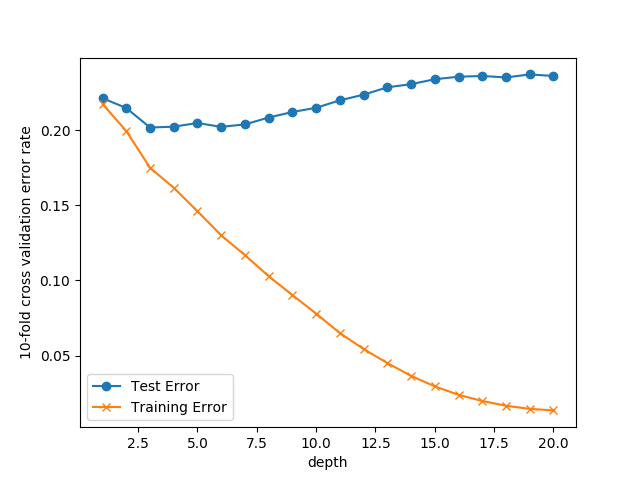
\includegraphics[width=\linewidth]{DecisionTree-CV.png}

\newpage
\item %4h
\solution{
Overall, it's clear that the Decision Tree performs better on this dataset than K-Nearest Neighbors, since the training and test errors for the Decision Tree were significantly lower on every trial. The trends of the Decision Tree learning curves, starting far apart but approaching each other as training data increases, indicates that the model obtained sufficient training data to perform well as the two lines converged.
}

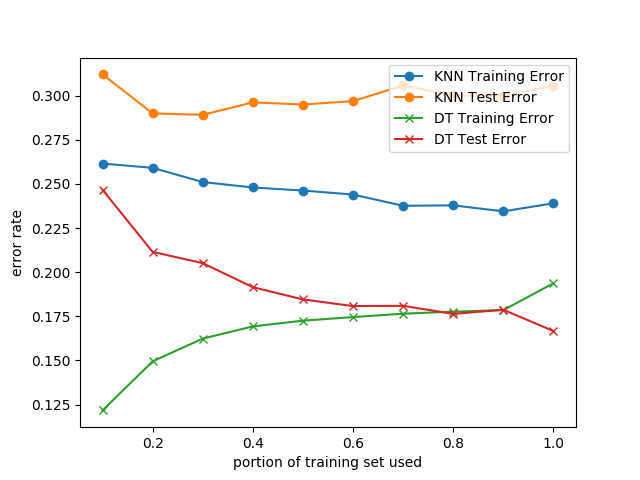
\includegraphics[width=\linewidth]{LearningCurves.png}

\end{enumerate}
\end{document}
